\subsection*{Bitcoin: A Peer-to-Peer Electronic Cash System}\cite{Nakamoto2008}

    \begin{itemize}
        \item Mangel: finanzelle Institutionen dienen als Third-Party -> Schwächen des vertrauensbasierten Modells
        \begin{itemize}
            \item Irreversible Transaktionen sind nicht wirklich möglich (können keine Schlichtungen bei Auseinandersetzungen vermeiden -> erhöht Transaktionskosten -> minimale Transaktionsgröße)
            \item Händler müssen aufpassen an wen sie verkaufen (z.B. mehr Informationen als eigentlich nötig sammeln)
            \item ein bestimmer Anteil an Fraud wird angenommen
            \item durch physische Währung vermeidbar, aber nicht elektronisch
        \end{itemize}
        \item basiert auf kryptographischen Beweisen anstatt Vertrauen
        \item zwei Entitäten können direkt Transaktionen durchführen
        \item Transaktionen sollen rechnerisch unpraktisch rückgängig sein -> Verkäufer vor Täuschung schützen, Treuhandmechanismen können einfach implementiert werden
        \item Lösung für das Double-Spend Problem
    \end{itemize}

\subsubsection*{Konzept}
    \begin{itemize}
        \item P2P verteilter Timestamp-Server, der rechnerische Beweise der chronologischen Reihenfolge der Transaktionen generiert
        \item so lange sicher, wie die "ehrlichen" Knoten gemeinsam mehr Rechenleistung als zusammenarbeitende Angreifer halten
    \end{itemize}

\subsubsection*{Transaktionen}
    \begin{itemize}
        \item elektronischer Coin = Kette digitaler Signaturen
        \item wird von einem Besitzer zum anderen transferiert, indem er einen Hash der vorigen Transaktion und den öffentlichen Schlüssel des nächsten Besitzers digital signiert den Hash dann am Ende des Coins anfügt
        \item Empfänger kann die Kette des Besitzes via Signaturen zurückverfolgen
        \item Problem: Empfänger kann nicht verifizieren, dass mit dem Coin nicht auch mehfach gezahlt wurde -> häufig: TTP zur Prüfung: Coin muss an Mint zurückgegeben werden, erzeugt neue - nur dieseknn vertraut werden, dass sie nicht mehrfach genutzt wurden
        \item Übertragen auf Bitcoin: der Empfänger muss sichergehen können, dass die vorigen Besitzer keine vorherigen Transaktionen signiert haben
        \item man muss also alle Transaktionen kennen (vgl. in der Rolle des Ausstellers/Mint)
        \item Transaktionen werden announced/veröffentlicht, benötigt System bei dem alle Beteiligten sich auf eine einzige Historie in der Reihenfolge, in der Transaktionen getätigt wurden, einige
        \item Empfänger benötigt Beweis zur Zeit der Transaktion, dass die Mehrheit der Knoten sich einig waren, dass dies die erste entgegengenommene Transaktionn gewesen ist.
    \end{itemize}
    \begin{figure}[H]
        \centering
        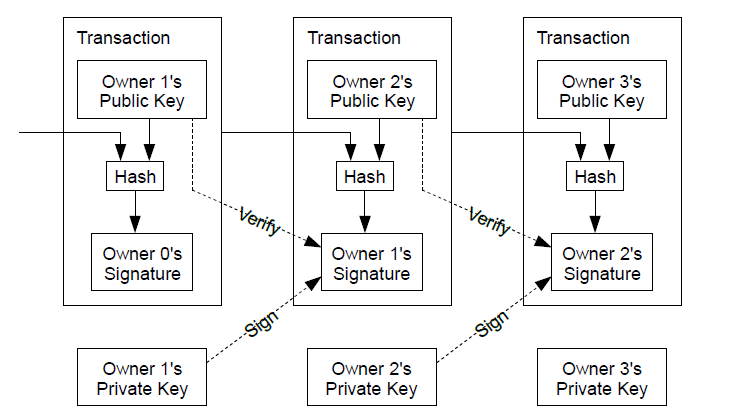
\includegraphics[width=0.7\textwidth]{paperNotes/bitcoin01.PNG}
        \caption{Coin}
        \label{figure:coin}
    \end{figure}

\subsubsection*{Timestamp Server}
    \begin{itemize}
        \item nimmt den Hash eines Blocks von Dingen und veröffentlicht den Hash (ähnlich Nachrichtenzeitung)
        \item Zeitstempel beweist, dass die Daten zu dem Zeitpunkt existierten, um in den Hash zu kommen
        \item Jeden Zeitstempel beinhaltet den Hash des vorigen Zeitstempels -> Kette (jeder zusätzliche Zeitstempel verstärkt die vorigen)
    \end{itemize}
    \begin{figure}[H]
        \centering
        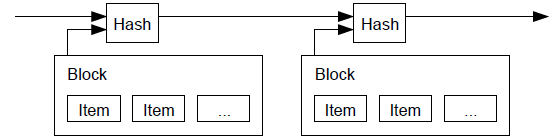
\includegraphics[width=0.7\textwidth]{paperNotes/bitcoin02.PNG}
        \caption{Block}
        \label{figure:block}
    \end{figure}

\subsubsection*{Proof-of-Work}
    \begin{itemize}
        \item Konzept: Wert scannen, der, wenn gehasht z.B. mit SHA-256 mit einer Anzahl von 0 Bits beginnt
        \item durschnittlicher benötigter Aufwand ist exponential zu der Anzahl von 0-Bits, die benötigt wird und kann durch einen einzigen Hash verifiziert werden
        \item POW: nonce im Block erhöhen bis ein Wert gefunden ist, der dem Block einen Hash mit den benötigten 0-Bits gibt
        \item sollte der POW erschöpft sein, kann der Block nicht verändert werden ohne die Arbeit nochmals zu verrichten -> da alle weiteren Blöcke verknüpft sind, ist die zu verrichtende Arbeit yum Ändern des BLocks um vieles mehr, da diese dann alle auf den Block folgenden beinhaltet
        \item löst ebenfalls das Problem: bestimme die Repräsentation in der Mehrheitsentscheidung
        \item wenn IP-Adresse = 1 Stimme, dann kann dies schnell durch die Allokierung vieler IP-Adressen untergraben werden -> POW bedeutet so viel wie 1 CPU = 1 Stimme. 
        \item Mehrheitsentscheidung ist repräsentiert durch die längste Kette (am meisten POW-Arbeit invenstiert)
        \item Kompensieren der immer schnelleren Hardware: durch gleitenden Mittelwert, welcher die mittlere Anzahl an Blöcken/Stunde anvisiert (wenn zu viele ->  höhere Geschwindigkeit)
    \end{itemize}
    \begin{figure}[H]
        \centering
        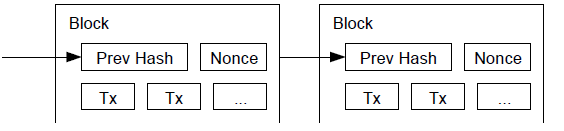
\includegraphics[width=0.7\textwidth]{paperNotes/bitcoin03.PNG}
        \caption{Chain}
        \label{figure:chain}
    \end{figure}

\subsubsection*{Netzwerk}
    Betreiben eines Netzwerks in folgenden Schritten:
    \begin{enumerate}
        \item neue Transaktionen werden an alle Knoten verbreitet
        \item jeder Knoten sammelt neue Transaktionen in einem Block
        \item jeder Knoten arbeitet daran einen schwierigen POW für seinen Block zu finden
        \item wenn ein Knoten einen POW findet, verbreitet er diesen BLock an alle anderne Knoten
        \item Knoten akzeptieren den BLock nur, wenn alle Transaktionen darin valide sind und noch nicht verbraucht wurden
        \item Knoten teilen ihre Akzeptanz des Blockes mit indem sie an dem nächsten Block in der Kette arbeiten und als vorigen Hash den des akzeptierten Blocks verwenden
    \end{enumerate}
    \begin{itemize}
        \item Knoten halten immer die längste Kette für die richtige und arbeiten daran diese zu verlängern
        \item zwei Knoten verbreiten verschiedene Versionen des nächsten Blocks gleichzeitig -> andere Knoten nehmen den ersten, den sie empfangen haben und arbeiten daran weiter, aber speichern den anderen Branch, falls dieser später länger wird
        \item Gleichtstand wird aufgebrochen, wenn der nächste POW gefunden wurde -> alle Knoten arbeiten an dem längeren Branch weiter
        \item Veröffentlichungen von neuen Transaktionen müssen nicht zwingend alle Knoten erreichen, es reichen "viele" um in einen Block zu kommen
        \item Veröffentlichungen von Blöcken tolerieren auch verlorengegangene Nachrichten -> wenn Knoten einen Block nicht empfängt wird dieser angefordert, wenn der nächste Block empfangen wird und bemerkt wird, dass ein Block fehlt
    \end{itemize}

\subsubsection*{Incentive/Motivation/Anreiz}
    \begin{itemize}
        \item nach Konvention: erste Transaktion eines Blocks ist eine Spezielle, die einen neuen Coin startet. Dieser ist im Besitz des Blockerzeugers. -> Anreiz für Knoten das Netzwerk zu unterstützen, sowie ein Weg, um erstmals Coins in den Umlauf zu bringen
        \item Analogie: ständiges Hinzugeben von neuen Coins in den Umlauf wie Goldschöpfer (Ressourcen a.k.a. CPU-Zeit und Elekrizität aufwenden -> Gold in den Umlauf birngen)
        \item Anreiz kann durch Transaktionskosten unterstützt werden: Wert nach der Transaktion < Wert vor der Transaktion -> Unterschied sind die Transaktionskosten, die zum Anreizwert des Blocks, der die Transaktion enthält addiert werden
        \item sobald dann eine bestimmte Zahl an Coins im Umlauf sind, kann der Anreiz komplett inflationsfrei in die Transaktionskosten übergehen
        \item kann dabei helfen die Knoten ehrlich zu halten -> wenn Angreifer mehr CPU-Stärke hat als die Ehrlichen -> entscheiden zwischen seinen Zahlungen zurückholen oder neue Coins generieren -> eher nach den Regeln mit neuen Coins spielen (sonst wird System unterlaufen und die Validität des eigenen Reichtumgs gefährdet)
    \end{itemize}
    
\subsubsection*{Festplattenspeicher wieder freimachen}
    \begin{itemize}
        \item wenn Coin unter genügend Blöcken vergraben ist, können die verbrauchten Transaktionen vor ihm verworfen werden
        \item um den Hash des Blockes nicht zu verwerfen, werden die Blöcke in einem Merkle-Baum gehasht -> nur dessen Root-Hash wird im Block-Hash gespeichert -> Zweige der Bäume können abgeschnitten werden, innere Hashes müssen nicht gespeichert werden
        \item einiges zur Speichergröße
    \end{itemize}
    \begin{figure}[H]
        \centering
        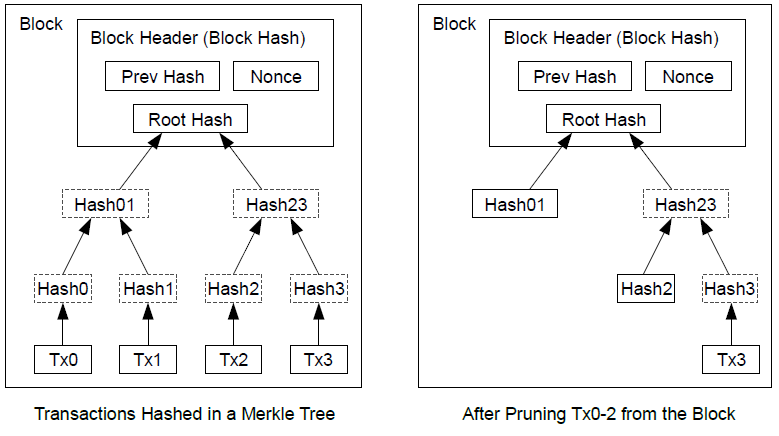
\includegraphics[width=0.7\textwidth]{paperNotes/bitcoin04.PNG}
        \caption{Speicher frei machen}
        \label{figure:prune}
    \end{figure}

\subsubsection*{Vereinfachte Verifizierung von Zahlungen}
    \begin{itemize}
        \item es ist möglich Zahlungen zu verifizieren ohne einen kompletten Netzwerkknoten zu betreiben
        \item Nutzer muss nur eine Kopie der Block-Header der längsten POW-Kette halten (bekommt man, in dem man Anfragen an Netzwerkknoten stellt bis er davon überzeugt ist die längste Kette zu haben und den Zweig des Merkle-Baums zu haben, welcher den Block mit dem Zeitstempel der zu verifizierenden Tranasktion enthält.
        \item kann also nicht die Transaktion selber prüfen, sondern kann erkennen, dass ein Netzwerknoten diese akzeptiert hat, wenn diese ienen Platz in der Kette hat (am besten dann, wenn danach noch andere Blöcke folgen -> wurde von mehreren Knoten akzeptiert)
        \item Verifizierung ist glaubwürdig, wenn ehrliche Knoten das Netzwerk kontrollieren
        \item Netzwerkknoten können Transaktionen selbst verifizieren
        \item Wenn ein Angreifer das Netzwerk überstimmt, kann die vereinfachte Methode durch vom Angreifer fabrizierte Transaktionen getäuscht werden -> Gegenmaßnahme: Alerts von Netzwerkknoten, wenn diese einen invaliden Block erkennen -> Nutzer lädt den kompletten Block und die vom Alert betroffenen Transaktionen neu
    \end{itemize}
    \begin{figure}[H]
        \centering
        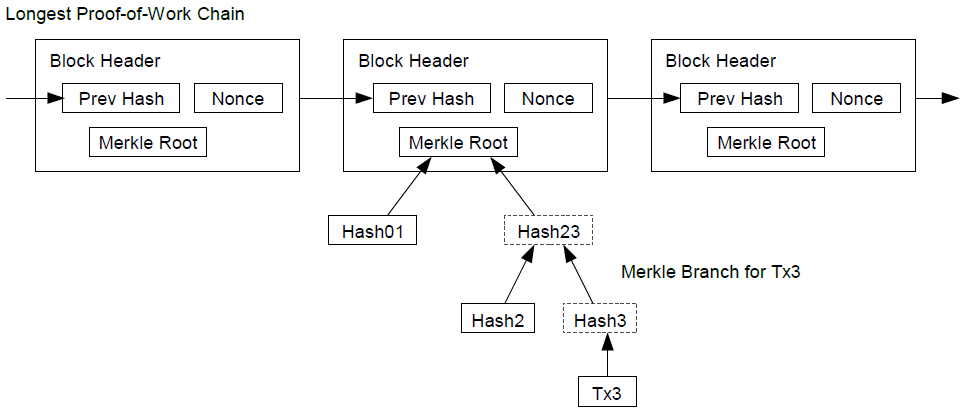
\includegraphics[width=0.7\textwidth]{paperNotes/bitcoin05.PNG}
        \caption{Transaktion verifizieren}
        \label{figure:verify}
    \end{figure}
    
\subsubsection*{Werte kombinieren und teilen}
    \begin{itemize}
        \item Separate Transaktion für jeden Cent im Coin sind unhandlich
        \item Transaktionen können mehrere In- und Outputs haben
        \item normal: einzelner oder mehrere Inputs und maximal zwei Óutputs (Zahlung und Rückgeld)
        \item 
    \end{itemize}
    
\subsubsection*{Privatsphäre}
    \begin{itemize}
        \item traditionell: Bank schränkt Zugriff auf Informationen auf TTP und die involvierten Parteien ein
        \item da alle Transaktionen öffentlich bekanntgegeben werden, wird die traditionelle Methode ausgeschlossen -> öffentliche Schlüssel sind anonym, ähnlich wie bei Börsen
        \item zusätzlich soll für jede Transaktion ein neues Schlüsselpaar verwendet werden, sodass mit den Schlüssel nicht auf einen Besitzer geschlossen werden kann
        \item Risiko bei mehrere Inputs einer Transaktion: deren Inputs gehören zum selben Besitzer
    \end{itemize}


\subsection*{Blockchains and Smart Contracts for the Internet of Things}\cite{Christidis2016}
    \subsubsection*{Einführung}
        \begin{itemize}
            \item ,,vertrauenslose`` Netzwerke \textrightarrow\ schellere Einigung
            \item Smart Contracts: selbstausführende Skripte, die auf der Blockchain "wohnen" \textrightarrow\ verteilte, stark automatisierte Workflows
        \end{itemize}
        
    \subsubsection*{Wie Blockchains funktionieren}
        \begin{itemize}
            \item verteilte Datenstruktur, die zwischen den Mitgliedern eines Netzwerkes repliziert und geteilt wird
            \item Knoten des Netzwerkes (Miner genannt) fügen validierte, gegenseitig abgemachte Transaktionen hinzu
            \item Blockchain beinhaltet das maßgebliche Hauptbuch von Transaktionen, welches festlegt wem was gehört
            \item auch ohne Cryptowährung möglich
            \item Log, dessen Einträgte als Blöcke mit Zeitstempeln zusammengefasst wurden
            \item jeder Block wird durch seinen kryptographischen Hash identifiziert und referenziert den Hash des vorigen Blocks (geordnete, zurückreferenzierendte Liste von Blöcken) \textrightarrow\ Link zwischen den Blöcken \textrightarrow\ chain of blocks \textrightarrow\ blockchain
            \item Jeder mit Zugriff kann die Blockchain lesen und daraus auf den aktuellen ,,World State`` der Daten, die auf dem Netzwerk ausgetauscht werden, schließen
            \item BC Network: Menge von Knoten (Clients), die mittels einer jeweils eigenen Kopie auf der selben BC operieren
            \item Knoten kann als Zugangspunkt für meherere verschiedene Nutzer in das Netzwerk genutzt werden \textrightarrow\ P2P-Netzwerk
                \begin{itemize}
                    \item Nutzer interagieren mittels eines Paares von öffentlichem und privatem Schlüssel
                    \item private: Transaktion signieren
                    \item öffentlich: Nutzer ist addressierbar
                    \item asymmetrische Kryptographie \textrightarrow\ Authentication, Integrity and Non-Repudiation im Netzwerk
                    \item jede signierte Transaktion wird durch den Knoten des Nutzers an alle Peers, die einen Hop entfernt sind, publiziert.
                    \item Benachbarte Peers stellen sicher, dass die eingehende Transaktion gültig ist bevor sie diese weiter verbreiten \textrightarrow\ irgendwann auf das ganze Netzwerk verteilt, ungültige Transaktionen werden verworfen
                    \item Die Transaktionen, die durch das Netzwerk innerhalb eines abgemachten Zeitraumes gesammelt und validiert wurden. werden sortiert und in einen "candidate Block" gepackt und mit einem Zeitstempel versehen \textrightarrow\ Prozess wird Mining genannt.
                    \item der minende Knoten veröffentlicht diesen Block dann wieder gegenüber dem Netzwerk (Auswahl des minenden Knotenns und der Inhalt des Blocks hängen vom Konsensmechanismus des Netzwerkes ab)
                    \item Die Knoten verifizieren, dass der vorgeschlagene Block: gültige Transaktionen enthält und via Hash den korrekten vorigen Block auf deren Kette referenziert.
                    \item Wenn beide Voraussetzungen erfüllt sind, wird der Block der Kette hinzugefügt und die enthaltenen Transaktionen ausgeführt, sodass World View aktualisiert wird. Sollten die Voraussetzungen nicht erfüllt sein, wird der Block verworfen
                    \item ein Schritt eines wiederkehrenden Prozesses
                \end{itemize}
            \item Vertrauen wird als entstehende Eigenschaft durch Interaktionen zwischen verschiedenen Teilnehmern im System erreicht
        \end{itemize}
        
    \subsubsection*{Konsens im Netzwerk erreichen}
        \begin{itemize}
            \item Knoten müssen sich einigen welche Transaktionen und in welcher Reihenfolge diese in dem neu-geminten Block aufgelistet werden
            \item falls nicht, entstehen Forks (Abspaltungen), also unterschiedliche Kopien der BC pro Benutzer \textrightarrow\ unterschiedliche Word States \textrightarrow\ Netzwerk kann keine authoritive Chronologie mehr halten bis der Abspaltung aufgelöst wurde \textrightarrow\ distributed consensus mechanism
            \item ideal: alle validierenden Knoten stimmen für die Reihenolge der Transaktionen ab und die Mehrheit entscheidet.
            \item bei offenem Netzwerk: wäre katastrophisch \textrightarrow\ Sybil attack (Identitäten fälschen, um die Mehrheit zu erlangen) \textrightarrow\ Mining rechnerisch teuer machen
            \item Leading zeroes bei Bitcoin - mehr = schwerer \textrightarrow\ POW \textrightarrow\ darf den nächsten Block formen, kann leicht verifiziert werden
            \item Hashfunktionen, die für POW genutzt werden: SHA-256, Blake-256, scrypt, Myriad
            \item Proof of Stake: weniger CPU-Berechnungen als POW, Wahrscheinlichkeit eines Knotens den nächsten Block zu minen ist proportional zur Balance des Knotens \textrightarrow\ eigene Vor- und Nachteile, Implementieren ist komplex
            \item in privaten Netzwerken: Nutzer werden über Whitelist verwaltet \textrightarrow\ POW wird nicht benötigt (kein Risiko eines Sybil-Angriffs) \textrightarrow\ keine ökonomische Anregung für Mining nötig \textrightarrow\ andere Konsensprotokolle sind möglich
            \item Practical Byzantine Fault Tolerance - Algorithmus: Lösung des Byzantinischen Generale-Problem, das in asynchronen Umgebungen wie dem Internet funktioniert
                \begin{itemize}
                    \item Protokoll mit drei Phasen
                    \item "Leader" Knoten, der als Block-Miner funktioniert, kann durch einen "View-Change" durch den Rest des Netzwerks via Abstimmung geändert werden - falls crashed oder sonstige Verhaltensauffälligkeiten aufweist (Byzantine Faults)
                    \item nimmt an, dass weniger als ein Drittel der Knoten Fehlerverhalten aufweisen \textrightarrow\ benötigt als mindestens 3xf + 1 Knoten
                \end{itemize}
            \item weitere Algorithmen: Tangaroa, Tendermint, Unique Node Lists (Ripple), Sieve (Hyperledger Fabric) mining diversity scheme (Multichain): whitelisted miners fügen Blöcke in Round Robin hinzu mit etwas Spielraum für gestörte Knoten etc.
        \end{itemize}
    
    \subsubsection*{Transferieren von digitalen Gütern auf einer Blockchain}
        \begin{itemize}
            \item Datenbanktabelle mit 3 Spalten: Asset Type, Owner/Counter-Party, Quantity/Amount - z.B. USD, Alice, 10 \textrightarrow\ Alice hat \$10
            \item Übertragung von Assets als Transformation von mehreren Zeilen in der Datenbank - als digitale Repräsentation
            \item digital repräsentierte Güter: Owner als public key, Alice erstellt Zeile mit Bob/2 aka Transaktion, sowie neue Zeile mit Alice/8, alte Zeile wird ,,gelöscht`` \textrightarrow\ keine gleichzeitigen Modifikationen auf einer Zeile bei Nebenläufigkeit
            \item Bob's Kontostand von Assets kann durch Aggregation der Zeilen Bob mit Type \$ berechnet werden
            \item Validierung: Transaktion auf eine existierende Zeile? Korrekt signiert, wird also diese Reihe dann gelöscht? Wurde diese Zeile bereits durch eine vorige Transaktion adressiert und validiert? (\textrightarrow\ double spend nicht möglich) Wurde die richtige Menge von Asssets in die neue Zeile übertragen? (Summe aller Inputs == Summe aller Outputs)
            \begin{figure}[H]
                \centering
                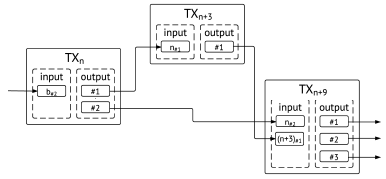
\includegraphics[width=0.7\textwidth]{paperNotes/chrisitidis201601.PNG}
                \caption{Transaktion mit mehreren Ein-/Ausgaben}
                \label{figure:transaction}
            \end{figure}
            \item neue Assets oder zusätzliche Items von bestehenden Assets werden als ,,besondere`` Transaktion eingeführt (generell durch einen ordentlich authorisierten Knoten)
            \item Carol erlaubt sich selbst neue Assets im Netzwerk auszuhändigen, lädt Alice und Bob ein. Beide sind damit einverstanden, dass Carol Assets ausstellen kann. Carol stellt 10 Assets aus und besitzt diese nun.
        \end{itemize}
        
    \subsubsection*{Funktion von Smart Contracts}
        \begin{itemize}
            \item 1994 von Nick Szabo eingeführt. Definition: ,,computergesteuertes Transaktionsprotokoll, das die Vertragsbedingungen ausführt``\cite{Szabo1996}
            \item Übersetzung von Vertragsklauseln in Code, der selbst in Hardware/Software eingebettet wird, um diese selbst durchzusetzen \textrightarrow\ möglich wenig Bedarf von vertrauten Vermittlern zwischen den den Parteien einer Transaktion und weniger Aufkommen von bösartigen oder unbeabsichtigten Ausnahmen
            \item bei BC: Skripte, die auf der BC gespeichert werden und von jedem Teilnehmer des Netzwerkes angesehen werden können (analog: Stored Procedures in einem relationalen Datenbanksystem
            \item haben eine einzigartige Adresse, werden über Transaktion mit deren Adresse getriggert \textrightarrow\ wird unabhängig ausgeführt
            \item können permissioned sein (z.B. nur Bob kann Contract ,,withdraw`` auf seine Adresse ausführen)
            \item hat eigenen Zustand und kann Assets auf der BC bei sich aufbewahren, in dem Tabellenmodel wäre ein SC also eine eigene Entität, die Zeilen löschen und hinzufügen kann
            \item BC untersützt das ,,kontobasierte`` Modell
            \item erlaubt es Geschäftslogik als Code auszudrücken
            \item ordentlicher SC sollte alle möglichen Endergebnisse des Contracts beschreiben
            \item Eine Trnsaktion ist eine ,,signierte Datenstruktur, die die Übertragung eines Wertes bezeichnet``\cite{Christidis2016}
            \item Bob sagt deutet mit einem SC z.B. an: wenn jemand mir 5 von X sendet, sende ich 10 von Y zurück
            \item SC sind deterministisch (gleicher Input \textrightarrow\ gleicher Output. Fall nichtdeterministisch, kein Konsens über das Ergebnis des SC im Netztwerk \textrightarrow\ idealerweise nichtdeterministische SC ablehen oder Sprache verwenden, die keine nichtdeterministischen SC erlaubt
            \item Da alle Interaktionen mit einem SC über signierte Nachrichten auf der BC verlaufen bekommen alle Teilehmer des Netzwerks eine kryptographisch verifizierbare Spur/Historie aller vom SC ausgeführter Operationen
        \end{itemize}
        
    \subsubsection*{Blockchain und \gls{iot}}
        \begin{itemize}
            \item zentralisiertes Modell hat hohe Instandhaltungskosten (Update Distribution) aus Sicht der Hersteller
            \item aus Verbrauchersicht: wenig Vertrauen, Geräte ,,reden mit zu Hause`` und den Ansatz von Sicherheit durch Transparenz
            \item Probleme können durch das skalierbarere, vertrauenslose P2P-Modell, das transparent funktionieren und Daten sicher verteilt kann, gelöst werden \textrightarrow\ BC
            \item Bsp: alle \gls{iot}-Geräte eines Herstellers laufen auf dem selben BC-Netzwerk. Hersteller nutzt einen Smart Contract, der es allen geräten erlaubt einen Hash des neusten Firmware-Updates auf dem Netzwerk zu speichern (entweder wird die Adresse des SC eingebacken oder finden es durch einen Discovery Service). Können den SC anfragen und so herausfinden, ob es ein neues Update gibt.
        \end{itemize}

\subsection*{MITM bei BLE ausmerzen via Kryptographie und Stenographie}\cite{Bapat2017}
    \subsubsection*{BLE}
        \begin{itemize}
            \item Link Layer Security via CBC-MAC und 128-Bit AES, 4byte Message Integrity Check appended to PDU, Counter gegen Replayangriffe, DOA - Empfänger verifiziert Signatur, weitere Keys blabla
            \item Vulns
                \begin{itemize}
                    \item Eavesdropping
                    \item MITM: Angreifer bekommt die gepairten Geräte dazu zu denken, dass sie getrennt seien -> zwei BT-Module (Master/Slave) -> Packet injection und authentication Attacks + Erlärung
                    \item DOS: v.a. Batterie aufbrauchen
                \end{itemize}
            \item Stenographie: Struktur der Nachricht wird nicht verändert (im Ggt. zu Kryptographie), sondern versteck die Nachricht so, dass ihre Existenz unbemerkt bleibt. Je nach Typ unterschiedliche Techniken wie man die Daten versteckt (Technisch, in Bildern, Audio, Video und linguistisch, in einem größeren Block Text- bspw. durch Formatierung, Rechtschreibfehler oder Ändern der Textgröße).
            \item vorgeschlagene Lösung für Smart Lock mit Android und Raspberry Pi via BLE: erst mit AES verschlüsseln, dann in ein Bild einbetten via BLE verwenden
        \end{itemize}

\subsection*{BC \& SC}\cite{Christidis2016} 
    \subsubsection*{Taxonomy}
        \begin{itemize}
            \item public/permission-less: jeder kannn beitreten
            \item private/permissioned: whitelist
            \item -> entscheidet, welcher Konsensmechanismus verwendet werden sollte, in public BC teuer und eine ökonomische Anregung wird normalerweise benötigt, private sinnvoll: kontrolliert, regulierte Umgebung oder höherer Durchsatz wie in einem öffentlichen
            \item wer Transaktionen durchführen oder minen kann: es müssen nicht alle TN Transaktionen durchführen, SC aufsetzen oder am Miningprozess teilnehmen können -> macht Sinn, wenn die Mitglieder des Netzwerks identifizierbar sind
            \item Bitcoin-Style Transaktionen oder SC (accountbasiert): BC nur für Transfer und Verfolgung digitaler Güter in Form von Tokens geeignet - accountbasiert kann beliebige Logik und verifizierbare Prozesse mit mehreren Schritten ausführen -> Kosten für Nebenläufigkeit und Durchsatz von Transaktionen, da keine Vorhersehbarkeit für spätere Zustände eines SC und evtl. weitere Trigger
        \end{itemize}
        
    \subsubsection*{BC und IoT}
        \begin{itemize}
            \item bietet geschickte Zahlungsmöglichkeit via Kryptowährung für z.B. Dienste -> Marketplace of Services between Devices
            \item Bsp: Gerät speichert Binary und verlangt Geld, um diese bereitzustellen, weitere Beispiele
            \item Jedes Gerät ein eigenes Bankkonto
            \item Slock.it: Smart Lock, Unlock via Device mit bestimmten Token, der via Ethereum eingekauft werden kann (Whisper P2P Protocol)
            \item Supply Chain Beispiel mit Container Tracking - entweder mit SC via signierten Nachrichten oder als Container-Token. Umsetzung z.B. via Tracker bei Stakeholder und Container, senden der Daten via IoT, useful: Mesh-Netzworks, deren Mitglieder jeweils einen Gateway für Internetzugang anbieten können -> low deployment costs
        \end{itemize}
        
    \subsubsection*{Deployment Considerations - Issues}
        \begin{itemize}
            \item lower transaction processing throughput \& higher latencies, v.a. bei öffentlichen Netzwerken mit POW
            \item kein Sharding, da jeder Knoten in Netzwerk die gleiche Aufgabe ausführt, v.a. bei Neztwerken mit SCs
            \item Privatsphäre: TN muss nicht alle Keys kennen, nur den der Partei auf der anderen Seite der Transaktion(bei privateneher doof, da sonst keine Zugriffskontrolle möglich ist)... jedoch sind alle Transaktionen öffentlich -> Analyse nach Identifikationsmerkmalen möglich. -> Mitigation Possibilities: Jedes Mal einen neuen Key für die Trx benutzen oder zumindest einen anderen Schlüssel pro Transaktionspartner
            \item bei privaten Netzwerken: ratsam nicht die gleich BC für alle Trx benutzen, falls ein anderer TN die Mehrheit erlangen könnte, in dem dessen Aktivität verfolgt wird -> exposure von Geräten minimal halten. BC nur mit den Entitäten aufsetzen, mit denen das Gerät zusammenarbeiten soll -> höhere Kosten für die Koordination, aber bessere Privatsphäre
            \item Transactional privacy (confidentiality): homomohpic Encryption, Zero-Knowledge Proofs -> ressourcenintensiv, Workaround: BC für einen bestimmten Prozess aufsetzen und danach wieder verwerfen
            \item Miner set betrachten oder festlegen: obwohl ein Miner keine Transaktion fälschen oder die Historie manipulieren kann, kann er neue gültige Transaktionen daran hindern in die BC eingefügt zu werden (Zensur). Byzantinische Knoten dürfen nur bis zu einem bestimmen maximalen Anteil auftauchen, bei mehr als de Schwellwert ist das Risiko der Zensur groß -> Miner-Knoten müssen sorfältig ausgesucht werden, sodass die Chancen geheimer Absprachen zwischen den Knoten möglichst gering sind - in privaten BC sollten Verträge unterschrieben werden
            \item legale Durchsetzbarkeit von SC sind im Moment limitiert. Sinnvoll, wenn im SC Referenzen auf einen Vertrag in RL sind (dual Integration): 
                \begin{enumerate}
                    \item SC einsetzen, dessen Adresse speichern und diese dann im echten Vertrag angeben
                    \item den korrespondierenden RL Vertrag Hashen, dessen Digest speichern und den RL Vertrag sicher ablegen
                    \item Trx an den SC senden. Der SC enthält den RL Vertrag in dessen Metadaten
                \end{enumerate}
            \item erwarteter Wert von tokenisierten Gütern. Problematisch bspw. wenn jemand einen Token gegen ein Gut im RL umtauschen will.
            \item Totale Autonomie ist ein doppelseitiges Schwert: Logik vorher inspizieren - Failsafe Mechanismen im Code, um Sackgassen vorzubeugen - Immutable System oder priviligierter Nutzer, der z.B, SC löschen/modifizieren kann?
            \item weitere Mechanismen, die die Funktionalität komplementieren: DNS, sichere Kommunikation(z.B. via telehash oder Whisper) und Dateiaustausch(P2P File System, IPFS)
        \end{itemize}